% ><><><><><><><><><><><><><><><><><><><><><><><><><><><><><><><><><><><><><><
%       Mines LaTeX Thesis Template. 
% ><><><><><><><><><><><><><><><><><><><><><><><><><><><><><><><><><><><><><><
% This template was written for pdfLaTex Compilers
\documentclass[letterpaper,10pt]{article} %% <-- INPUT: Font size below, change the number to 10, 11 or 12pt

% ------------------------------------------------- Packages & Setup
\usepackage{csm-thesis}         % Proper Thesis Formatting. This requires the 'csm-style-files' directory

\usepackage{array}              % For inserting large multi-page tables
\usepackage{longtable}

\usepackage[numbers]{natbib}    % For proper citations
\usepackage{hyperref}           % For referencing though out the document. Can change, look at user manual how to change
\usepackage{pdflscape}          % For inserting landscape-mode objects 
\usepackage{amsmath}            % For matrices
\usepackage{listings}           % For inserting programming code
\usepackage{rotating}           % For inserting sideways tables and figures
\usepackage{lipsum}             % For dummy text. You can remove this once you have remove all of the example text. 

\usepackage{my-Equations}       % Where I define frequently used equations or symbols for easy use

% For using row-spanning and column-spanning in tables:
%\usepackage{multirow}


% For using helvetica instead of Computer Modern
% \usepackage{helvet}
% \renewcommand{\familydefault}{\sfdefault}
% ~~~~~~~~~~~~~~~~~~~~~~~~~~~~~~~~~~~~~~~~~~~~~~~~~~~~~ Place To Look For Figures
% This tells the pdf builder where to look for the figures that are added in the document
% you can add more paths if you wish, example:
% \graphicspath{{./figures/}{./figures/try-me}}
\graphicspath{{./in/figures/}}

% ><><><><><><><><><><><><><><><><><><><><><><><><><><><><><><><><><><><><><
%       GENERAL USER INFO: Title, Authors, Advisors...
% ><><><><><><><><><><><><><><><><><><><><><><><><><><><><><><><><><><><><><
% ~~~~~~~~~~~~~~~~~~~~~~~~~~~~~~~~~~~~~~~~~~~~~~~~~~~~~  TITLE
\title{
    Example of how to use the Colorado School of Mines\\
    Thesis/Dissertation \LaTeX{} template to help\\
    future graduate students with\\
    the formatting. \texorpdfstring{H$_2$O}{Water}
    }

% ~~~~~~~~~~~~~~~~~~~~~~~~~~~~~~~~~~~~~~~~~~~~~~~~~~~~~ PERSONAL INFORMATION
\degreetitle{Master of Science}     % Degree Title like Master of Science or Doctor of Philosophy
\discipline{Engineering Systems}    % Area of research, eg. Applied Physics
\department{Physics}                % Your department, eg. Physics

\author{Graduate A. Student}        % your NAME, don't forget your middle names.
\advisor{Dr. Primary A. Advisor}    % your Advisor, put Dr. in front if they have a PhD them selves!
\coadvisor{Dr. Secondary B. Advisor}% if you have a co-advisor, otherwise Comment out/remove the line
\dpthead{Dr. Big Boss}{Department Head Title}    % department head name & title. eg. \dpthead{Dr. Uwe Greife}{Professor and Department Head}

\begin{document}
% ><><><><><><><><><><><><><><><><><><><><><><><><><><><><><><><><><><><><><
%       FRONT MATTER
% ><><><><><><><><><><><><><><><><><><><><><><><><><><><><><><><><><><><><><
% If you do not want any of the following 'optional' items, either comment 
%   out those lines, or remove them from the document. Or if you do not have
%   any Figures, Tables, Symbols, or Abbreviations you can remove those lists.

\frontmatter                       % Leave this line here, it sets the formatting 
% requirements for the front matter of the document
\maketitle\newpage                 % >>>>>>>>> Title Page (required) <<<<<<<<<
\makecopyright{\the\year}\newpage  % >>>>>>>>> Copyright Page (optional) <<<<<<<<< 
\makesubmittal\newpage             % >>>>>>>>> Signature Page (required) <<<<<<<<<

% >>>>>>>>>>>>>>>>>>>>>>>>>>>>> Abstract (required) <<<<<<<<<<<<<<<<<<<<<<<<<<<<<
\begin{abstract}
    Here is the place where you will be adding an abstract for your document. The abstract should be between 200-300 words. The abstract is checked, and if your work count exceeds the 350 words it will produce and error. 

\lipsum[3]

\lipsum[1]
    % you can also directly type your abstract here if you prefer.
\end{abstract} \newpage

% >>>>>>>>>>>>>>>>>>>>>>>>>>>>>>>>>>>>>>> <<<<<<<<<<<<<<<<<<<<<<<<<<<<<<<<<<<<<<<

\tableofcontents\newpage        % >>>>>>>>> Table of Contents (required) <<<<<<<<<<<
\listoffigures\newpage          % >>>>>>>>> List of Figures (if applicable) <<<<<<<<
\listoftables\newpage           % >>>>>>>>> List of Tables (if applicable) <<<<<<<<<

% >>>>>>>>>>>>>>>>>>>>>>> List of Symbols (if applicable) <<<<<<<<<<<<<<<<<<<<<<<
% \ShowSymbolFirst                      % un-comment to show the symbols on the left of the list.
\listofsymbols*                         % the * puts the list in alphabetical order
\listofsymbols{General Nomenclature}    % calling a sub list
\newpage

% >>>>>>>>>>>>>>>>>>>> List of Abbreviations (if applicable) <<<<<<<<<<<<<<<<<<<<
\listofabbreviations*                  % the * puts the list in alphabetical order
\newpage

% >>>>>> Define Your Symbols and Abbreviations In the File Under 'supporting-files'
% You can add them any where in the text, but it is good to keep it in the same place.
% >>> Symbols
\addsymbol{Average radius of cylindrical shell}{$c$}
\addsymbol{activation energy of oxidation reaction of a-C in excited state}{$E^{\ast}_{act}$}

% >>> Symbols >> General Nomenclature
\addsymbol[General Nomenclature]{absorption cross section}{$\alpha_{\sigma}$}

% >>> Abbreviations
\addabbreviation{Colorado School of Mines}{CSM}
\addabbreviation{Bio Force Gun, Model 9000}{BFG9000}
\addabbreviation{Mammoth Armed Reclamation Vehicle}{MARV}
\addabbreviation{Stone of Jordan}{SoJ}
\addabbreviation{Field flow fractionation-inductively coupled plasma-mass spectrometry}{FFF-ICP-MS}

% >>>>>>>>>>>>>>>>>>>>>>>>>> Acknowledgments (optional) <<<<<<<<<<<<<<<<<<<<<<<<<
\begin{acknowledgments}
    I would like to thank and acknowledge $<$advisor$>$ $<$family$>$ $<$funding sources$>$ $<$committee$>$.
    %Write an acknowledgement that is appropriate to you and your work. You may decide who you want to include.
\end{acknowledgments} \newpage

% >>>>>>>>>> Dedication (optional) <<<<<<<<<<
% >>>>>>>>>>>>>>>>>>>>>>>>>>>>>>>>>>>>>>> <<<<<<<<<<<<<<<<<<<<<<<<<<<<<<<<<<<<<<<
% >>>>>>>>>>>>>>>>>>>>>>>>>>>>>>>>>>>>>>> <<<<<<<<<<<<<<<<<<<<<<<<<<<<<<<<<<<<<<<
\begin{dedication}
    For those that shall follow after.
    \addsymbol{hello}{$\cdots$}     %<-- you can add symbols and abbreviations anywhere in the text but it is good to keep them organized in one spot!
\end{dedication}\newpage


% ><><><><><><><><><><><><><><><><><><><><><><><><><><><><><><><><><><><><><><><><
%                   BODY: All Chapters and Sections
% ><><><><><><><><><><><><><><><><><><><><><><><><><><><><><><><><><><><><><><><><
\bodymatter     % Leave this line here, it sets the formatting requirements for the front matter of the document

% You can directly add you chapter text into this document. But to keep organized you
% are advised to separate you chapters into their own files, as this example shows
\chapter{Introduction}\label{chap:intro}

This is where you would place a fun and thoughtful introduction. For example I could address why it is so important that I am working on this Thesis \LaTeX{} Template? Well, it is probably so that future students that take on the challenge of writing their thesis in \LaTeX{} can get through the formatting a lot quicker, in that they don't have to worry about it at all.

Here I will also add some tips: (1) Keep everything organized by 'Type'. Note that all the chapters are added in separate files in the 'chapter' directory/folder. This is such that you can stay better organized. Similarly all the figures are in the 'figure' directory, feel free to make sub folders for each chapter, and all the supporting files such as the references or the abbreviation and symbol lists are in their own folder. 

(2) As you start working on this document try and keep the formatting to the end, because every time you change the text, figures or tables might move, and it is just easiest to leave that till the end. Lastly (3) this document and the accompanying files are to help beginners and experts, so if you are comfortable just go a head and get going. There is always the help guide to fall back on, and if you save a copy of the original files you can always go back and look what I presented to you.

There are some hidden chapters that are uncommented (with the \% in front of them) with a lot of figure and table examples that can be use full for you if you are not sure for to scale or add them properly. Relax, and good luck.
\chapter{My first chapter with some good content\label{chapTwo}}

After creating every new chapter or heading you can add a paragraph or more of text, or you can move right into a heading or subheading.

\subsection{Level 1}\label{sec:firstSection}
This is what a subsection title looks like with some text following. Here is a tip: Stay consistent. This counts for how you write your headers (all mayor words capitalize or only the first word). 
Below are some equations with some simple math here are three different ways to reference equations: (1) using ref  gives \ref{eqn:energy}, (2) using eqref leads to \eqref{eqn:Maxell1}), (3) and using the template defined Eqref gives \Eqref{eqn:Evalue}. You can not just use option (1) without indicating you are referencing an equation. Choose one and stick with it, they want you to be consistent in the way you reference Tables, Figures and equations alike. Automatically 'Table' and 'Figure' are added in fort of a reference number when you use ref\{\} for tables and figures (see in later chapters).

\begin{align}
    E =&\, m c^2 \label{eqn:energy}\\
    \nabla \times \bE =&\, -\frac{\partial {\bf B}}{\partial t} \label{eqn:Maxell1}
\end{align}
beginning a sentence right after the equation tells the documents that the paragraph is continuing and this sentence does not start with any indent. 

\begin{align}
	{\left[\begin{matrix}
	A_{11} & A_{12}\\ 
	A_{21} & A_{22}
	\end{matrix}\right]} {\bf v}=\lambda {\bf v}
	\label{eqn:Evalue}
\end{align}

We can now add a sub-sub section. This is also an example of an equation that is mid paragraph. If you eliminated the space between the math environment and the next line, then there should be no indent of the line right after the equation.

\subsubsection{Level 2}

This is what a sub-subsection looks like with some text following. \lipsum[2]

We can now add a sub-sub-sub section. But before we do that I need to add some text to check if the (a) ragged right is working, and (b) if the sub-sub-sub section will be pushed to the next page if the sub heading and 2 lines don't fit on the page. Ta-Da it works.


\paragraph{Level 3}

This does not look appealing, so you are discourage going "three deep" with headings. This does not look appealing, so you are discourage going "three deep" with headings.
\subsection{Here is an example of placing a subsub-section right after the sub-section}
\subsubsection{Here is the title of my subsub-section. I will be referencing the current chapter number}
The current chapter number is \ref{chapTwo}.
\chapter[This is a long title to check the proper spacing in the
Table of Contents and inverse pyramid on the chapter page. Lets see if it works properly. What if I add enough text so that there are like three or four lines here, does it change the way it looks.]{This is a long title to check the proper spacing in the
Table of Contents and\newline
inverse pyramid on the chapter page. Lets see if it works properly. What if\newline
I add enough text so that there are like three or four lines here,\newline
does it change the way it looks.}



\subsection{A Figure}
Here we have a section to show off one of the xkcd comics. \ref{fig:xkcd1} shows one of the comics showing the actual size of a number compared to the perceived size of a number. 

\begin{figure}[ht]
    \centering
    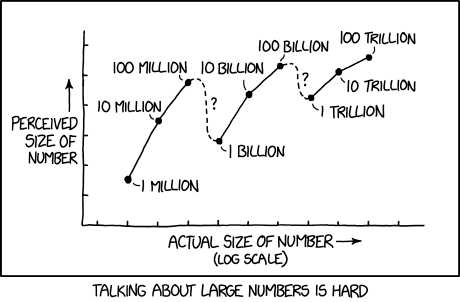
\includegraphics[width=0.7\textwidth]{image-01-million_billion_trillion.png}
    \caption{The trend of actual versus perceived size of a number. \cite{cite-munroe_2018}. We are also
    going to add a relatively long caption to check if the List of Figures works properly at the beginning of the document.}
    \label{fig:xkcd1}
\end{figure}
%Make sure to get permission to include any figures that you did not create, or indicate the open license. See guidelines in C-Appendix.tex

\subsection{Citing and referencing things}
On other figure shown in \ref{fig:phd-Comics1} shows a comic form \cite{cite-cham_2009}. 
If you want to group citations into one go, something you might do in the back ground section, you can do this by grouping multiple sources in your bibtex in the same 'cite' \cite{cite-A,cite-B,cite-C, cite-munroe_2018}.

You can also reference chapter, subsections or appendices al long as you place the label properly. Here I will reference you to see Appendix~\ref{sec:longtable} to check out how to add "longtabes" into your document, another example of that is shown in a hidden chapter on tables.
If you think there was something important in a previous section that you can reference them back with, Section \ref{sec:firstSection}. Or reference a chapter like Chapter \ref{chap:intro}.

Foot notes are allowed depending on the department you are working with. Please check with your advisor if you should be adding foot notes or not. Just so you have an example here is a footnote\footnote{here is a footnote}.

\csmfigure{phd-Comics1}{image-02-phd092809s.png}{5in}{"Vacation Relaxation?" by Jorge Cham
www.phdcomics.com. A nice comic form PHD Comic's. Learn more about the figure input notation in the Figure chapter, or in the hand book.}


Filler Text. \lipsum[4]

\subsection{Here is a test of a really long sub-header title that should automatically follow the rules for set for the Temple Guidelines and check if it properly shows up in the table of content. }

Here is a paragraph of filler text. \lipsum[2]
here is an extra sentence

% \addtocontents{toc}{\vspace{31\baselineskip}} % This line moved the Chapter 5 TOC entry to the next page to be with it's subheadings.

\chapter{Your Journal Paper Title Goes Here \label{sec-JA-Title1}}

\begin{center}
    Modified from a paper to be published in The Journal of ABC\footnote{Reprinted with permission of J. of ABC, 25(1), 41-45.}.
    
    Jane Jones\footnote{Graduate student and Associate Professor, respectively, at the Colorado School of Mines \label{note1}}$^,$\footnote{Primary researcher and author}, Sam Smith\footnote{Different Institution and position}, Ann Adams$^{\ref{note1},} $\footnote{Author for correspondence}
\end{center}

\subsection{Abstract}

This is the abstract that is part of the paper.  At the bottom of this page, beneath a 1.5" to 2" footnote line, can be footnotes with details of permission granted by the publisher of the paper, the author's titles and institution names, the relative contributions of each of the authors, et. If the abstract does not completely fill the page, the introduction also starts on this page. There are no page breaks between the different sections within the paper.

\subsection{Introduction}

The text of the introduction starts on the same page as the abstract, as long as there is room for at least two lines of text beneath the heading (This \LaTeX{} template should look for this automatically.) The headings within this chapter will match the style used in the rest of the thesis. All pages of text within the paper are completely filled in.

\subsection{Permissions}
Make sure you have checked the journal permissions about reproducing your paper in your thesis. Make sure you put these permissions in the Appendix \ref{sec-Apx-C}.

\subsection{The next section of the paper}
A lot more information from the paper that is being added into this dissertation. I would add figure, tables and other materials the same way as I have been in the other section of the dissertation. The big difference between this and the other chapters is the very top with the Journal and authors centered on the page.

Here is another paragraph that is just filler text. \lipsum[1]
\chapter{This is the title of a paper included in a thesis}

\begin{center}
    Reproduced with the permission for The Journal of ABC. \thefootnote[1]{text}
    
    Jane Jones, Sam Smith, Ann Adams
\end{center}

\subsection{Abstract}

This is the abstract that is part of the paper. If the abstract does not completely fill the page, the introduction also starts on this page. There are no page breaks between the different sections within the paper.

\subsection{Introduction}

The text of the introduction starts on the same page as the abstract, as long as there is room for at least two lines of text beneath the heading (This \LaTeX{} template should look for this automatically.) The headings within this chapter will match the style used in the rest of the thesis. All pages of text within the paper are completely filled in.

The next chapter shows another example with some foot notes for the authors, and the permission form the journal. Here is another quick sentence to make this paragraph look longer than it actually is, and not adding any new information for you to use.

% % Extra Example Chapters If you want to See Special Cases with Table, Figure, or Equation formatting
\chapter{Examples of Figures}
\label{cha:important-chapter}
This chapter shows you some examples of figures, such as subfigures,  big, and landscape figures.


\subsection{Just a figure}
As the subsection header states it is just a figure, \ref{fig:Strongbad}. But in the code it does not look like the regular 'figure' input. There is a function that allows you to input a figure, and only have part of the caption shown in the table of content, go ahead and compare the label of \ref{fig:Strongbad} below and the one that popped up in the table of content.

\csmlongfigure{Strongbad}{image-05photo_library_management.png}{2in}{This section of the citation will appear in the List of Figure}{ and this section is added to the citation in the text \cite{cite-xkcd_2017-anotherOne}.}

This function is useful when you have really long figure captions, and you don't need to show all of the description in the table of content.

Now I will add a figure (\ref{fig:CutvsFloatBarrier}) that will be place in the next section somewhere. Lets see what happens when I use Float Barrier.

\begin{figure}[ht]
	\centering
	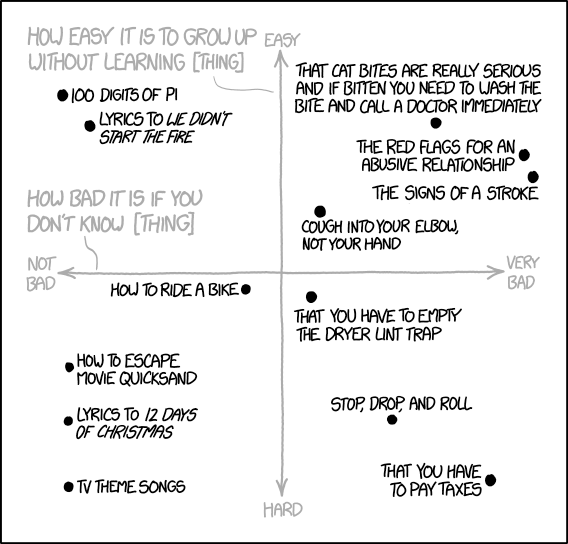
\includegraphics[width = 0.5\textwidth]{image-03.png}
	\caption{Here is a figure that will cut through the next section.}
	\label{fig:CutvsFloatBarrier}
\end{figure}

\FloatBarrier

\subsection{Sub-figures}

Note that both \ref{fig:fsm} and \ref{fig:fsm-2} show the same two figures with sub plots but look different in layout. Also look at where you place the 'label' in the figure, because you can also call one of the subplots, example are \ref{fig:fsm-pirates} and \ref{fig:fsm-pirates2}. The next paragraph is a bunch of non information, only to show where the two figures are going to naturally place themselves.

\begin{figure}
	\centering
	\subfigure[Blue Light with Interference Filter]{
		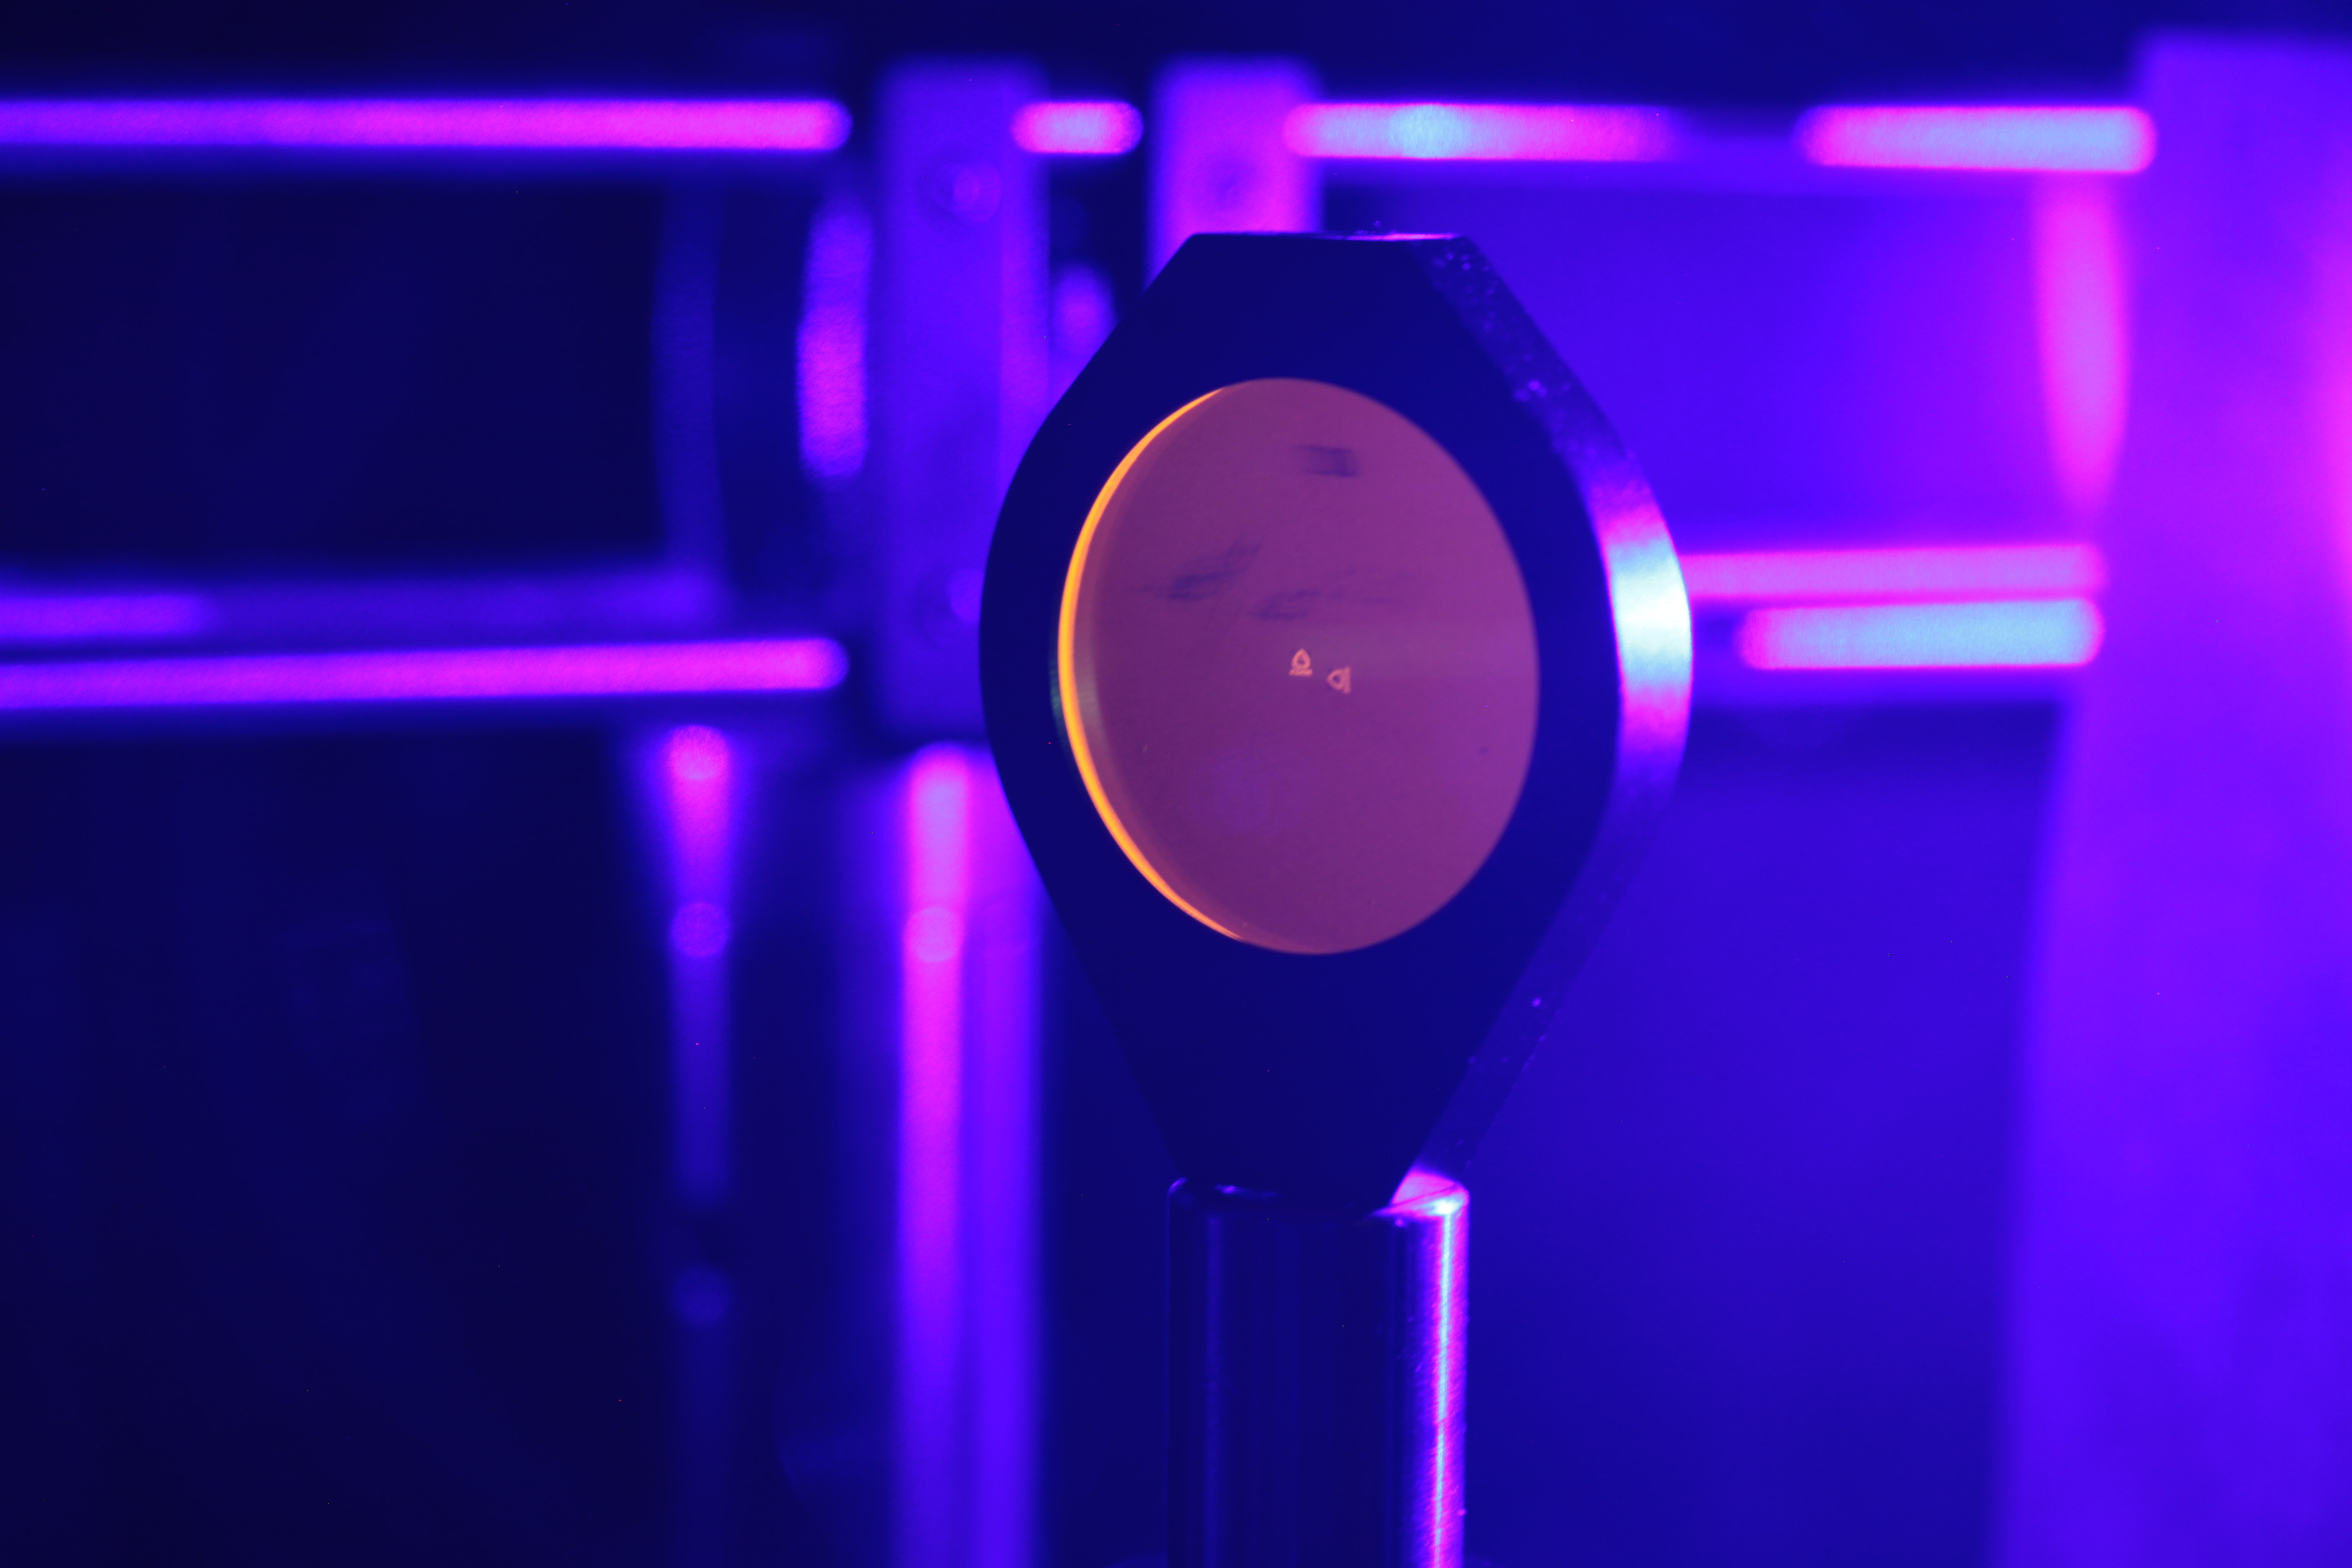
\includegraphics[width=4in]{IMG_2375.JPG}
	} \\
	\subfigure[Cool Sparks]{
		\resizebox{4in}{!}{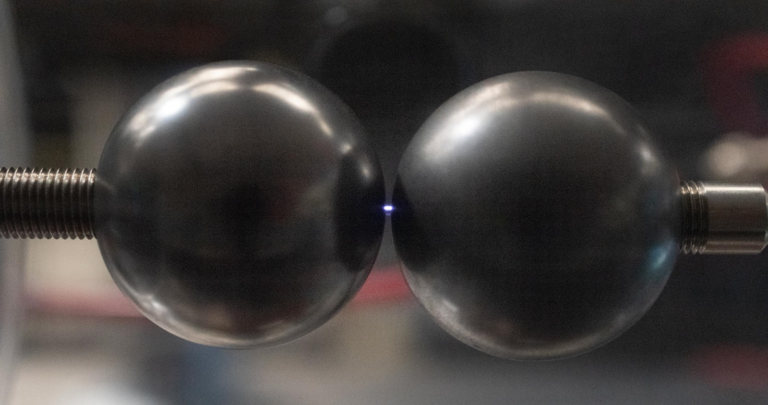
\includegraphics{/try-me/ESD_1600-768x405.png}}
		\label{fig:fsm-pirates}
	}
	\caption{\label{fig:fsm} Here are two images from the Durfee Research Group (a) A reflective object with something engraved in the center \cite{cite-schrama_2019-blue}. (b) A electrostatic discharge event occurring in air taken with a long exposure camera  \cite{cite-schrama_2019}}
\end{figure}

\lipsum[3]

\lipsum[4]

\begin{figure}[ht]
	\centering
	\subfigure[Blue Light with Interference Filter]{
		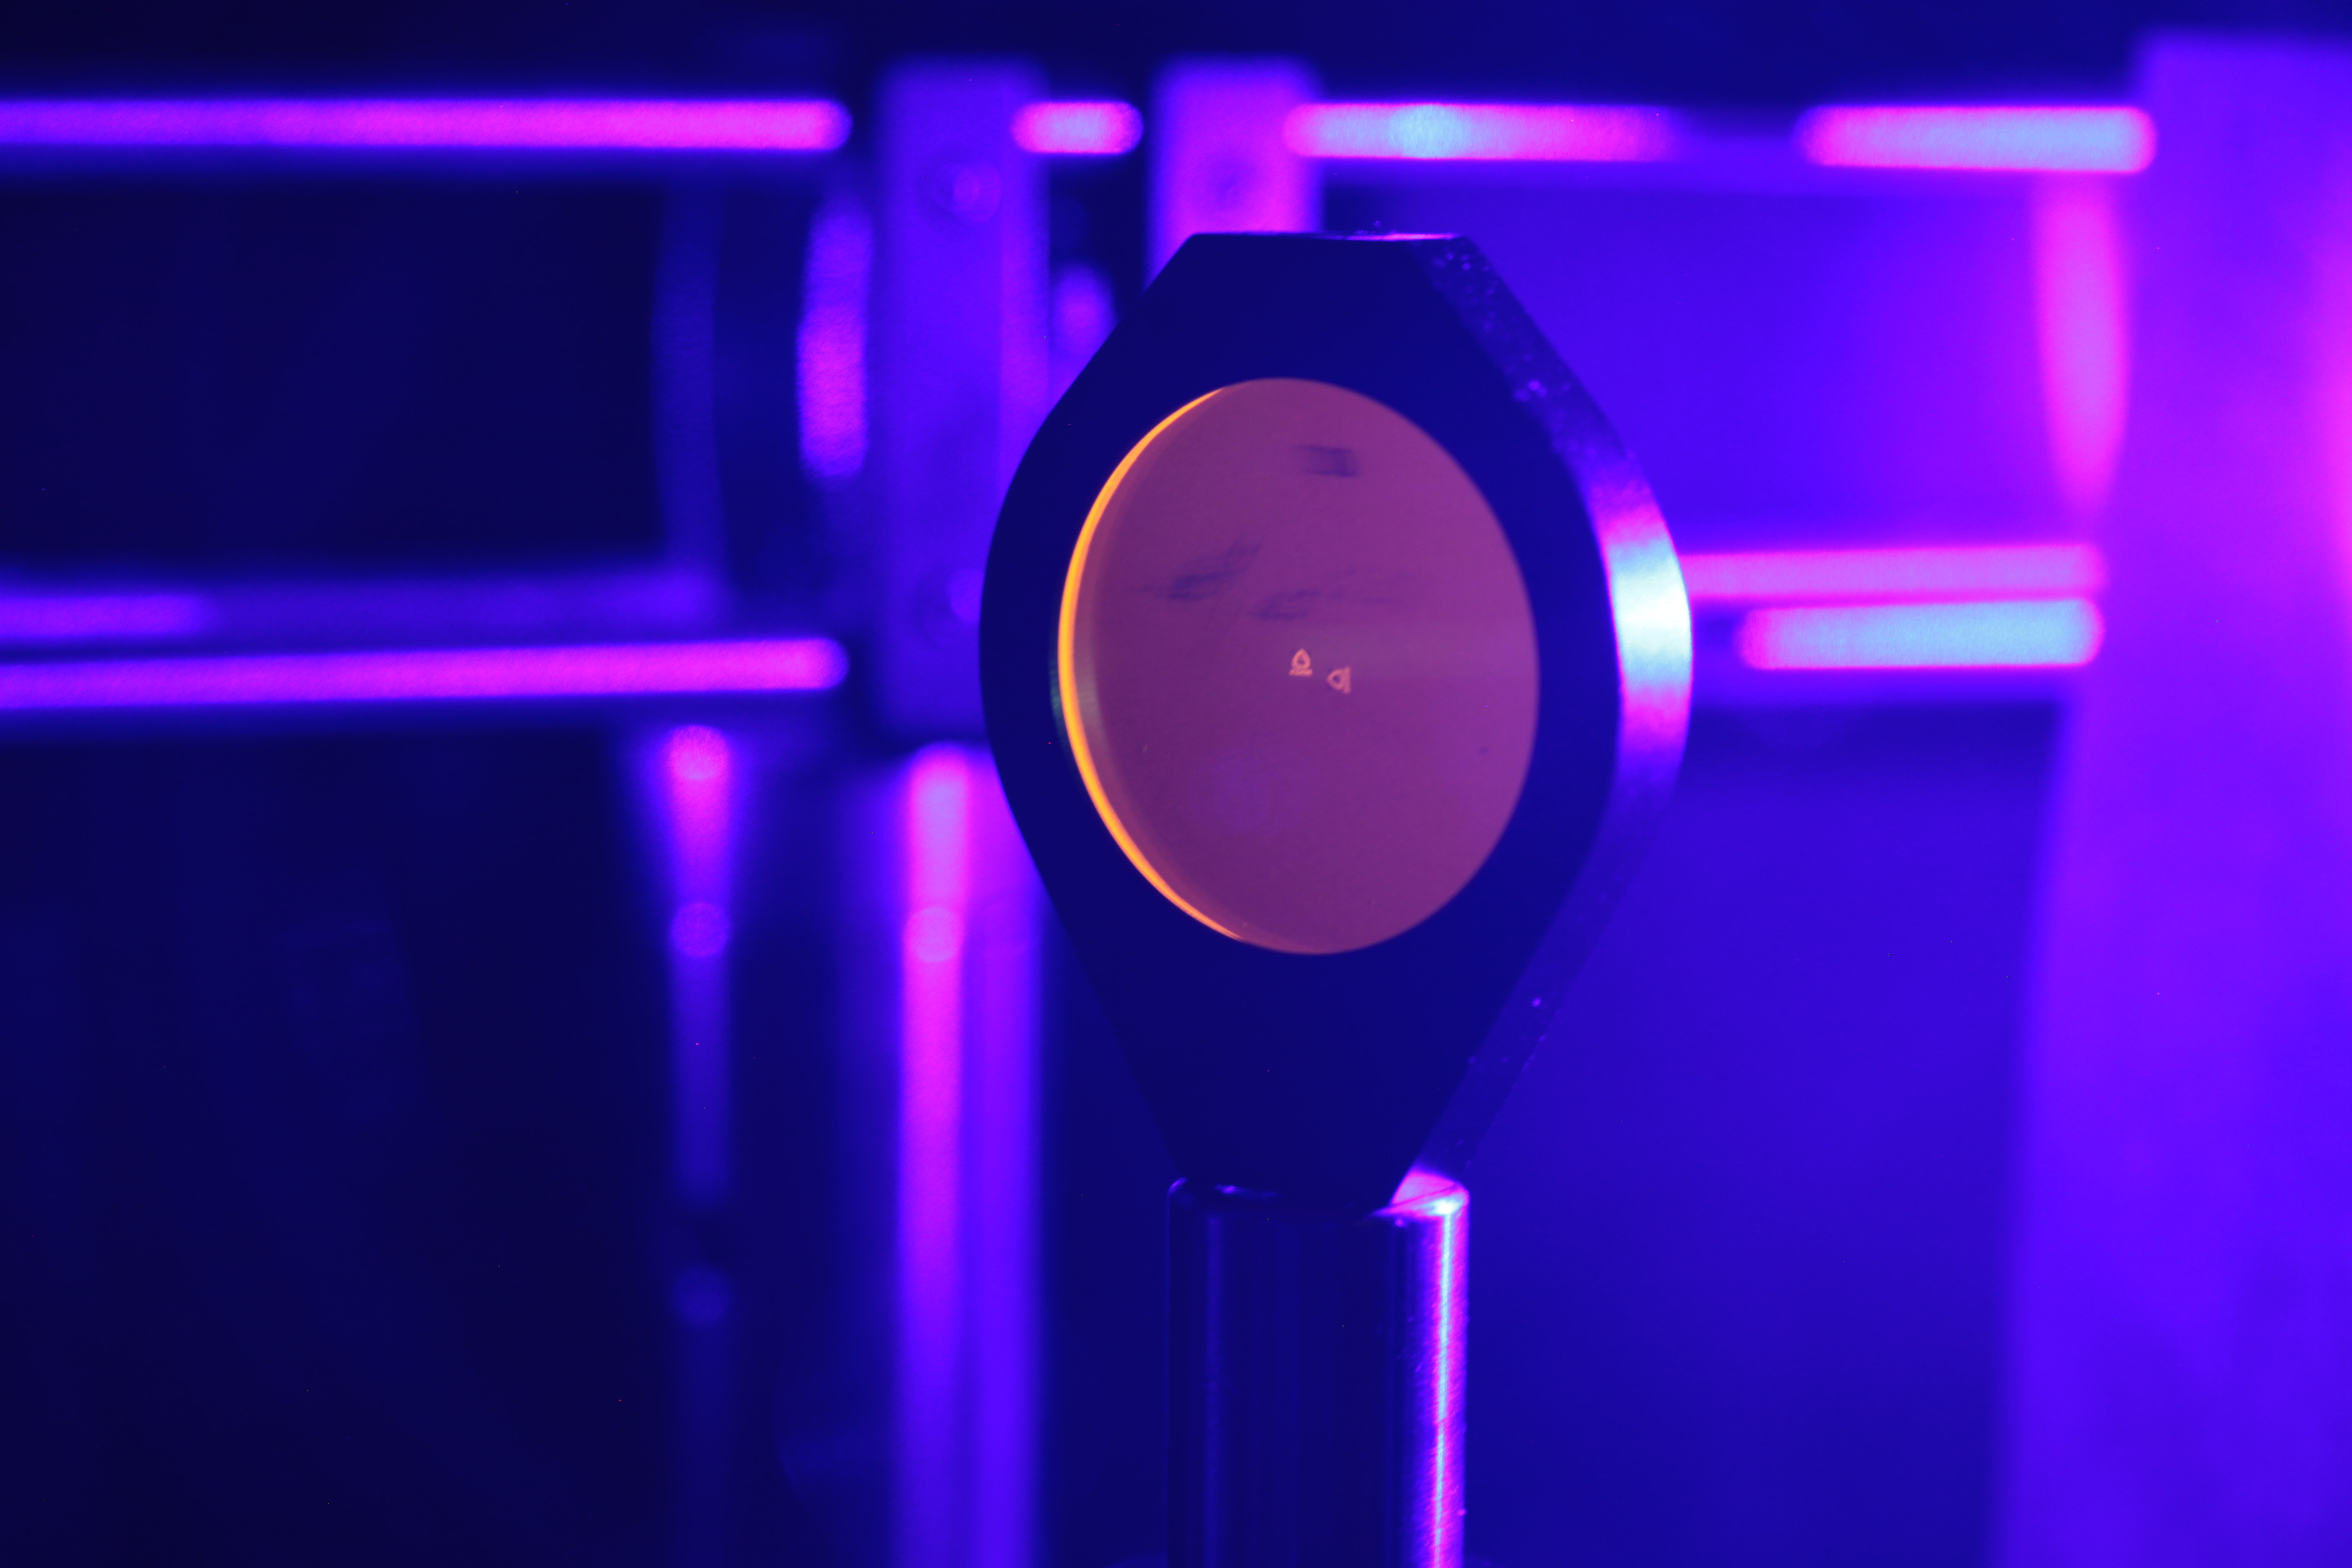
\includegraphics[width=2.5in]{IMG_2375.JPG}
		\label{fig:fsm-pirates2}
	} ~
	\subfigure[Cool Sparks]{
		\resizebox{2.5in}{!}{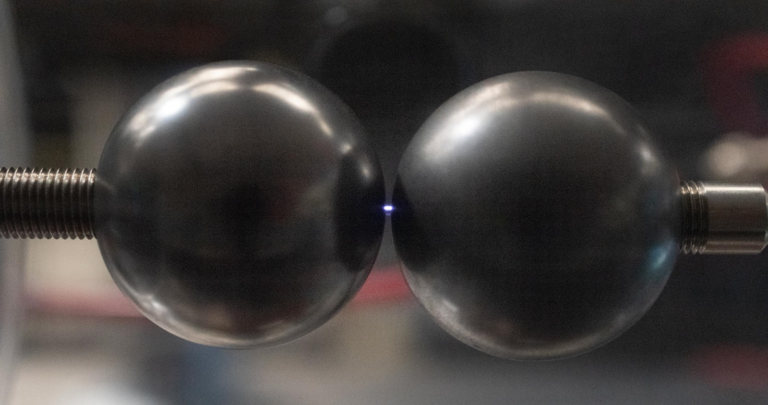
\includegraphics{/try-me/ESD_1600-768x405.png}}

	}

	\caption{\label{fig:fsm-2} Here are two images from the Durfee Research Group (a) A reflective object with something engraved in the center \cite{cite-schrama_2019-blue}. (b) A electrostatic discharge event occurring in air taken with a long exposure camera  \cite{cite-schrama_2019}}
\end{figure}


Notice the the figure with the stacked images places itself on its own page. This figure is greater than 50\% of the page, so if you leave of any placement tags (like [ht]) then most of the time the figure gets moved to it's of page.

\subsection{Landscape Figure}
There is also an example of a really big image following soon that takes up more than 50\% of the page and is in Landscape mode \ref{fig:hallo}. Note that the text wrap does not work around these landscape images, as it did for the above subplot, because Section \ref{sec-Important} should be right after this line. This means you need to think about where you place these landscape figures (or tables).

\begin{landscape}
	\centering
	\begin{figure}[ht]
		\centering
		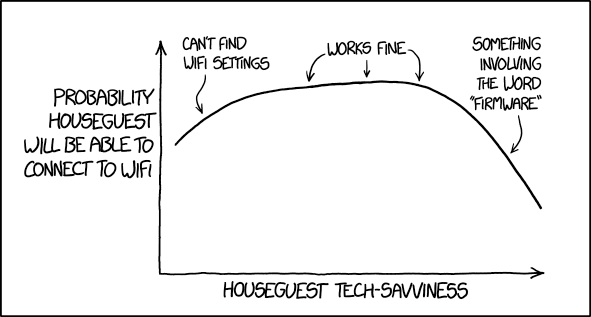
\includegraphics[width=\linewidth]{image-04.png}
		\caption{This is an example of a landscape page filled by a picture.}
		\label{fig:hallo}
	\end{figure}
\end{landscape}

\subsection{Here is an example that does not always work} \label{sec-Important}
We thought that was the end! But here I have placed a figure, \ref{fig:hallo2}, and it should pushes itself to its own page after this page is filled up all the way. If you comment out the paragraph between here and the figure you will see that the figure is placed wrong (and got rid of the [p] on the figure).

\lipsum[1]

\begin{figure}[p]
	\centering
	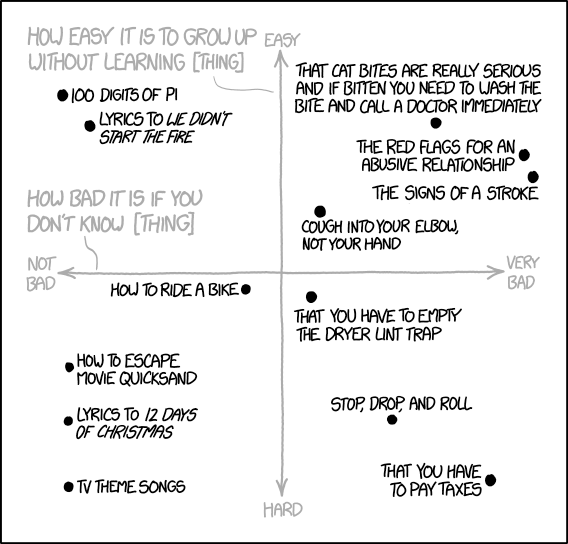
\includegraphics[width = \textwidth]{image-03.png}
	\caption{This figure will show after the current page has ended and only contain this figure on the page. \cite{cite-xkcd_2016}}
	\label{fig:hallo2}
\end{figure}

\lipsum[2]

\lipsum[3]

\lipsum[1]

Here is an example of a caption and a other thins \ref{fig:WayToBig}

\clearpage

\begin{figure}[p]
	\centering
	\caption{Here is a really long caption for the figure that will follow on the next page. So I have to make this caption really long. I can get this system to work but unfortunately the user will have to pay extra attention to the text wrapping because it will not do it one its own !!! This is very important. The figure is actually outside of the figure environment. So Clear the page, then insert the caption and label in the figure environment, and then clear the page again. This way you can add the [p] placement marker which will center the caption vertically on the page. Next add the figure after the second clear page with only include graphics and not in any figure environment. The image is one made by the author of this template document, Claudia Schrama, where a Moku:Lab instrument is used to analyze a circuit using the frequency response analyzer function. }
	\label{fig:WayToBig}
\end{figure}

\clearpage

\vspace*{\fill}
\begin{center}
	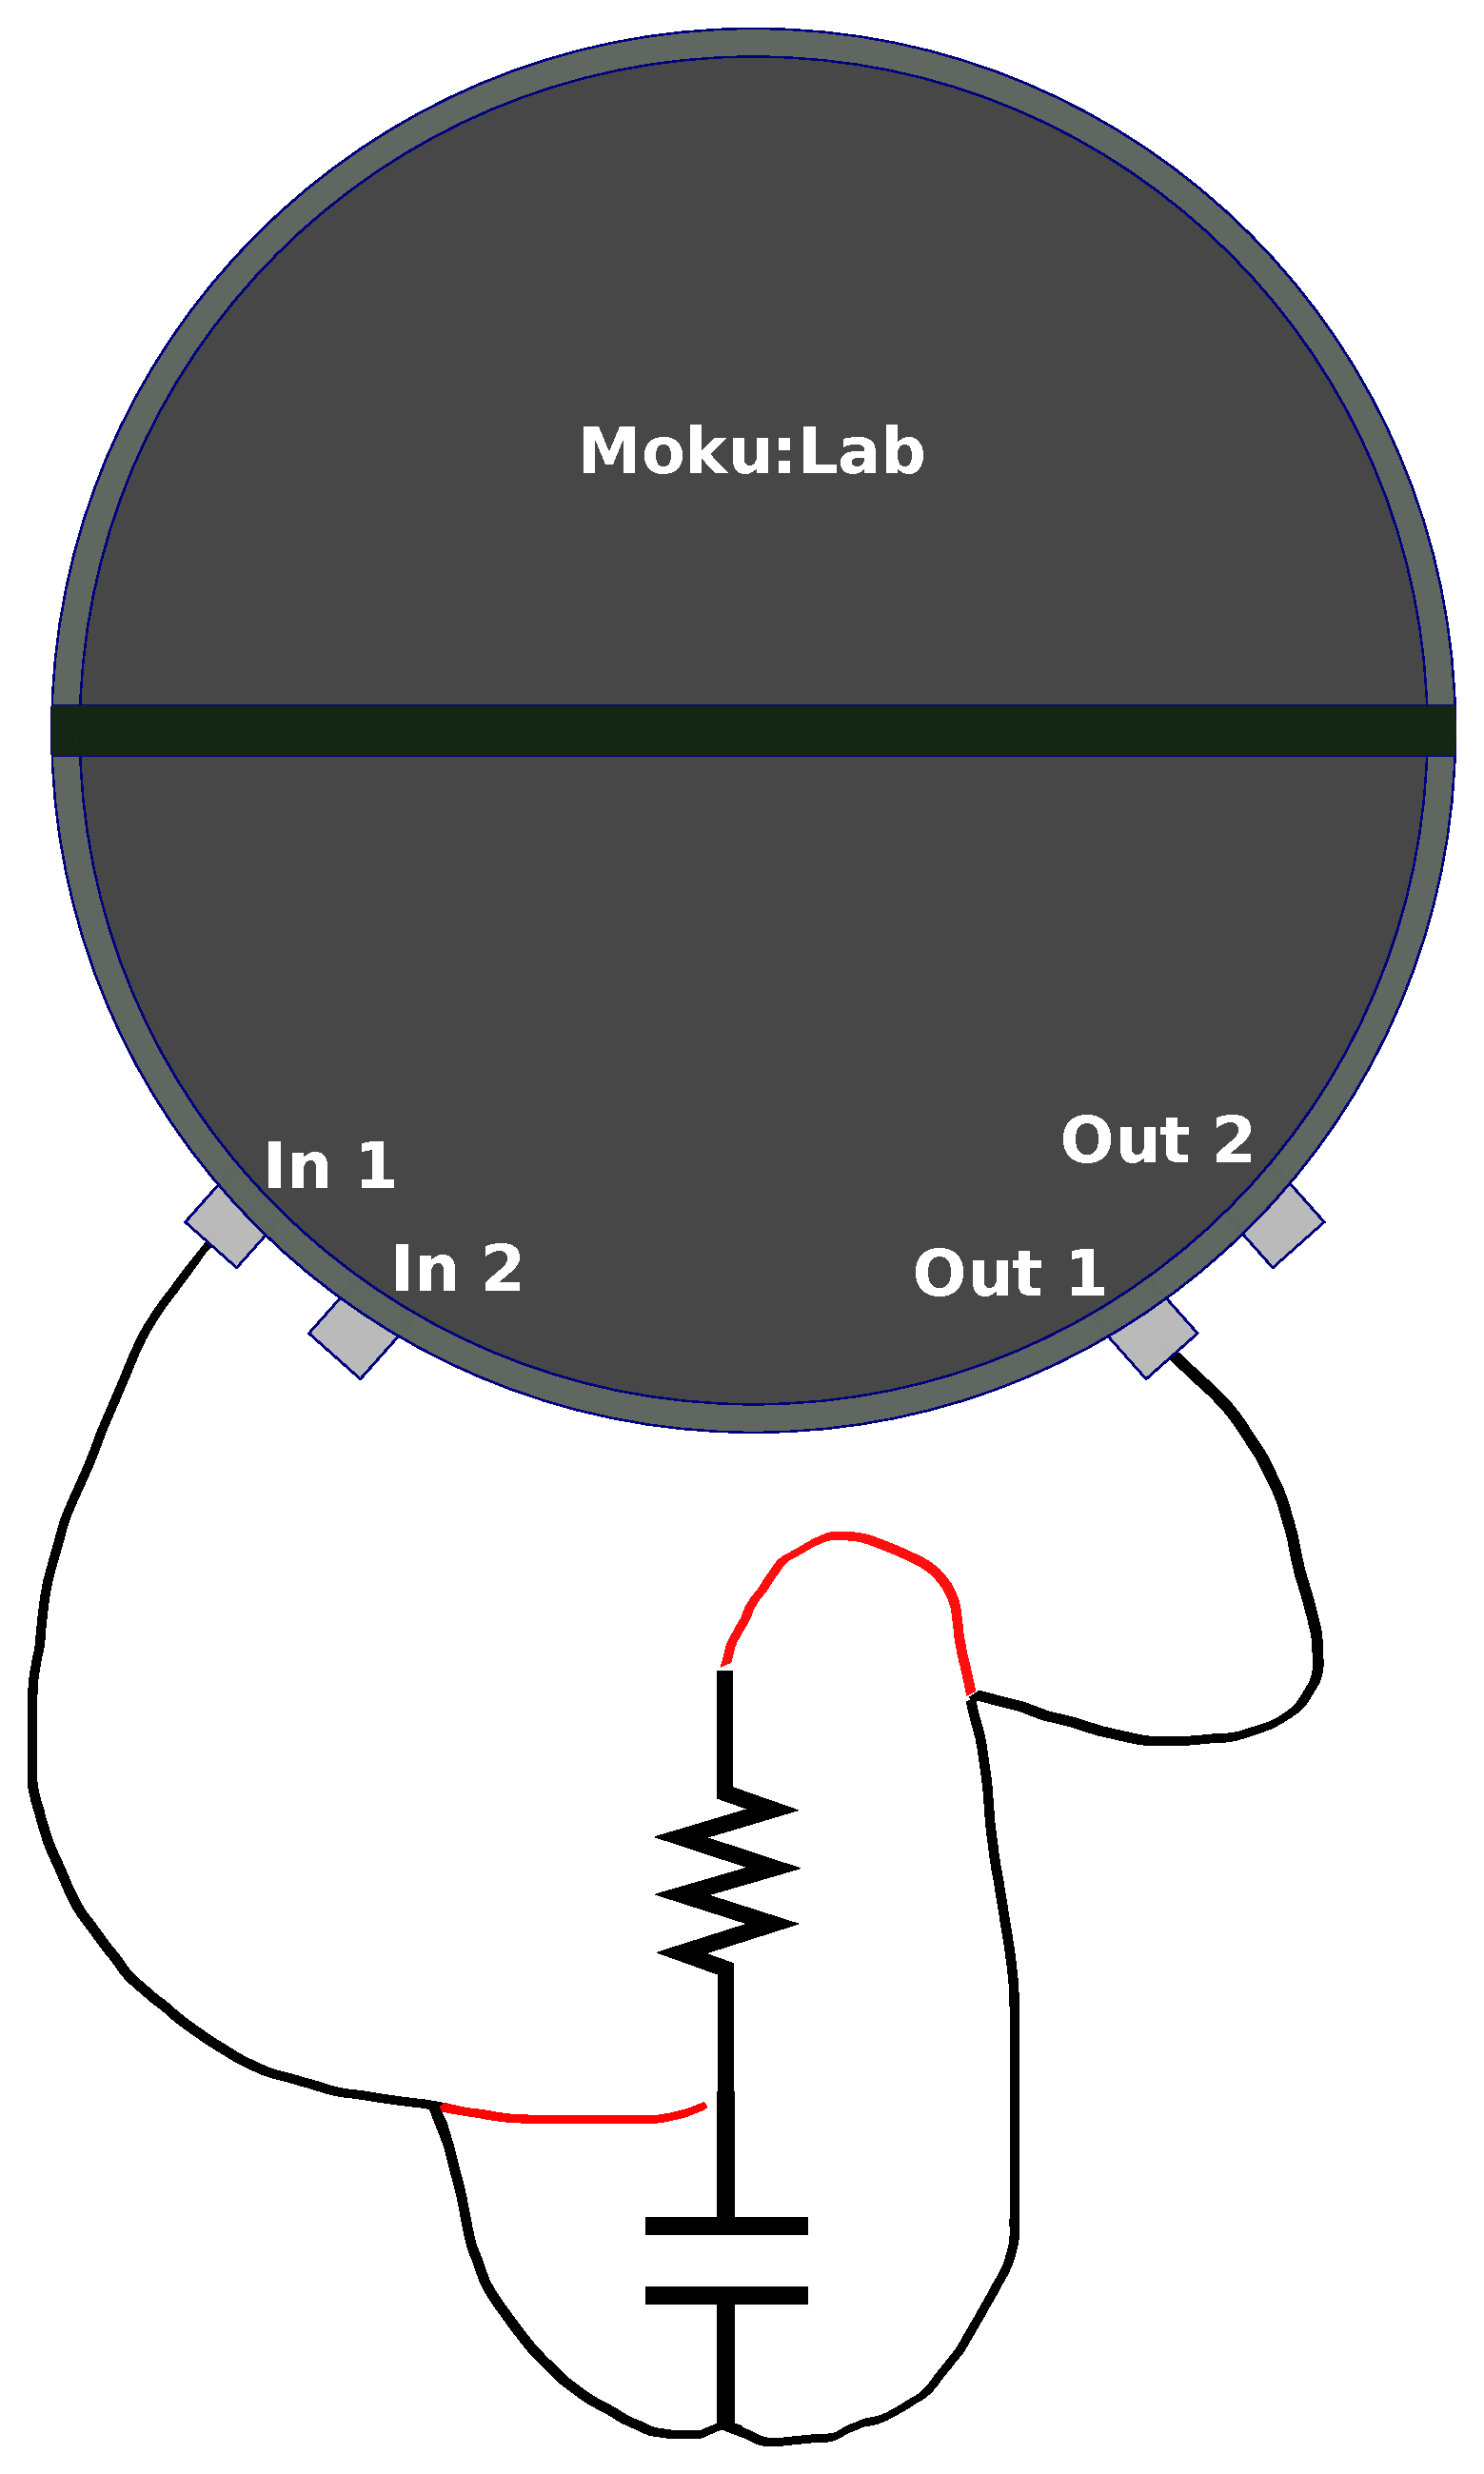
\includegraphics[height =0.9 \textheight]{20120-04-16-YoutubeLiquidInstuments.pdf}
\end{center}
\vspace*{\fill}

\clearpage


% \csmsplitfigure{yep}{Caption This}{!}{image-03.png}

\chapter{Examples of Tables}
This chapter gives you a few examples of Tables, including a landscape table.

\subsection{Just a Table}
Are you really still reading this? Okay, then check out \ref{tab:magic}! Is it not just magical. But in all seriousness you do not have to read most of the text in this chapter. Most of the text by now is filler text, showing you what things should be looking like from the way the school wants you to format your dissertation. 

\begin{table}
	\caption{\label{tab:magic} A table of tabular goodness. A lot of information in this heading to check if we get the proper response at the beginning of the document in the List of Tables}
	\begin{center}
		\begin{tabular}{|c|c|c|}
			\hline
			& B & b \\
			\hline
			B & BB & Bb \\
			\hline
			b & Bb & bb \\
			\hline
		\end{tabular}
	\end{center}
\end{table}


\subsection{Big table check}
Here is a lot of filler text to check that the figure is pushed after the page and then follows that later on. Here is a lot of filler text to check that the figure is pushed after the page and then follows that later on. Here is a lot of filler text to check that the figure is pushed after the page and then follows that later on. Here is a lot of filler text to check that the figure is pushed after the page and then follows that later on. Here is a lot of filler text to check that the figure is pushed after the page and then follows that later on. Here is a lot of filler text to check that the figure is pushed after the page and then follows that later on. Here is a lot of filler text to check that the figure is pushed after the page and then follows that later on. Here is a lot of filler text to check that the figure is pushed after the page and then follows that later on. Here is a lot of filler text to check that the figure is pushed after the page and then follows that later on. Here is a lot of filler text to check that the figure is pushed after the page and then follows that later on. Here is a lot of filler text to check that the figure is pushed after the page and then follows that later on. 

Now I will place a table (should be larger, but this is just showing the code works) on the next page because it could be to big. \ref{tab:my_labelTable}


\begin{table}
    \centering
    \caption{Table that should take up more than 50\% of the page to stand on its own. Note that it is automatically placed on it's own page when leaving off the placement (eg. [ht] is removed after \textbackslash begin\{table\})}
    \label{tab:my_labelTable}
\begin{tabular}{lcrcl}
\hline \T\B
Long Table & Big Table & 50\% of the page & Other & And another \\ \hline
1          & 2         & 3                & 4          & 5           \\
A          & B         & C                & D          & E           \\
6          & 7         & 8                & 9          & 10          \\
a          & b         & c                & d          & e          \\
11         & 21        & 31               & 41         & 51          \\
\textbf{A} & \textbf{B}& \textbf{C}       & \textbf{D} & \textbf{E}  \\
61         & 71        & 81               & 91         & 101         \\
\textbf{a} & \textbf{b}& \textbf{c}       & \textbf{d} & \textbf{e} \\
111        & 211       & 311              & 411        & 511         \\
\textit{A} & \textit{B}& \textit{C}       & \textit{D} & \textit{E}  \\
611        & 711       & 811              & 911        & 1011        \\
\textit{a} & \textit{b}& \textit{c}       & \textit{d} & \textit{e}  \\
1          & 2         & 3                & 4          & 5           \\
A          & B         & C                & D          & E           \\
6          & 7         & 8                & 9          & 10          \\
a          & b         & c                & d          & e          \\
11         & 21        & 31               & 41         & 51          \\
\textbf{A} & \textbf{B}& \textbf{C}       & \textbf{D} & \textbf{E}  \\
61         & 71        & 81               & 91         & 101         \\
\textbf{a} & \textbf{b}& \textbf{c}       & \textbf{d} & \textbf{e} \\
111        & 211       & 311              & 411        & 511         \\
\textit{A} & \textit{B}& \textit{C}       & \textit{D} & \textit{E}  \\
611        & 711       & 811              & 911        & 1011        \\
\textit{a} & \textit{b}& \textit{c}       & \textit{d} & \textit{e}  \\ \hline
\end{tabular}
\end{table}

\addsymbol{I have added a symbol in the Table Chapter}{$\nabla \lambda$}


Afghanistan Albania Algeria Andorra Angola Antigua and Barbuda Argentina Armenia Australia Austria Azerbaijan The Bahamas Bahrain Bangladesh Barbados Belarus Belgium Belize Benin Bhutan Bolivia Bosnia and Herzegovina Botswana Brazil Brunei Bulgaria Burkina Faso Burundi Cabo Verde Cambodia Cameroon Canada Central African Republic Chad Chile China Colombia Comoros Congo, Democratic Republic of the Congo, Republic of the Costa Rica Côte d’Ivoire Croatia Cuba Cyprus Czech Republic Denmark Djibouti Dominica Dominican Republic East Timor (Timor-Leste) Ecuador Egypt El Salvador Equatorial Guinea Eritrea Estonia Eswatini Ethiopia Fiji Finland France Gabon The Gambia Georgia Germany Ghana Greece Grenada Guatemala Guinea Guinea-Bissau Guyana Haiti Honduras Hungary Iceland India Indonesia Iran Iraq Ireland Israel Italy Jamaica Japan Jordan Kazakhstan Kenya Kiribati Korea, North Korea, South Kosovo Kuwait Kyrgyzstan Laos Latvia Lebanon Lesotho Liberia Libya Liechtenstein Lithuania Luxembourg Madagascar Malawi Malaysia Maldives Mali Malta Marshall Islands Mauritania Mauritius Mexico Micronesia, Federated States of Moldova Monaco Mongolia Montenegro Morocco Mozambique Myanmar (Burma) Namibia Nauru Nepal Netherlands New Zealand Nicaragua Niger Nigeria North Macedonia Norway Oman Pakistan Palau Panama Papua New Guinea Paraguay Peru Philippines Poland Portugal Qatar Romania Russia Rwanda Saint Kitts and Nevis Saint Lucia Saint Vincent and the Grenadines Samoa San Marino Sao Tome and Principe Saudi Arabia Senegal Serbia Seychelles Sierra Leone Singapore Slovakia Slovenia Solomon Islands Somalia South Africa Spain Sri Lanka Sudan Sudan, South Suriname Sweden Switzerland Syria Taiwan Tajikistan Tanzania Thailand Togo Tonga Trinidad and Tobago Tunisia Turkey Turkmenistan Tuvalu Uganda Ukraine United Arab Emirates United Kingdom United States Uruguay Uzbekistan Vanuatu Vatican City Venezuela Vietnam Yemen Zambia Zimbabwe

\subsection{Table That Spans Two Pages}
Here is an example of a big table that spans two pages, I this case it is in Landscape mode. The table,
\ref{tab:longtable1}, needs to be placed properly in the text such that there is not to much white space left on the page before it. This type of formating should be left till you are almost done with the capter, else you will constantly be editing the format, while you sould be focusing in the conten.
\begin{landscape}
\begin{longtable}{|>{\centering}p{1.02in}|>{\centering}p{1.15in}|>{\centering}p{1in}|>{\centering}p{0.7in}|>{\centering}p{0.7in}|>{\centering}p{0.67in}|>{\centering}p{2.55in}|} %
    \caption{A multipage table example to show people what to do, in case they have a really long table\label{tab:longtable1}}\\ 	\hline
	\endfirsthead % Remove this line to use the main header for the first page
	\hline
	one & two  & three & four  & five  &  six  & seven % These are the headers that show up on the following pages
	\endhead
	Item & Color & Fruit or Veggie & Flower      & Common Item\footnote{This was the best category that I could come up with} & Spice     & Closest Object to Me (Detail) \T\B \tabularnewline \hline 
    1 & White  & Cauliflower& Petunia    & Towel & Asafoetida Powder & The page of the PDF on the screen, for this document. It is showing this table as it is being filled out with more useless information. \tabularnewline \hline \Tn \Bn
    2 & Yellow & -          & Sunflower  & Sun   & Japanese Curry Powder  & A dish towel, as you read this table (i hope you are not) you will notice that I am in by apartment. It is one of those super absorbent ones.\tabularnewline \hline
    3 & Orange & Orange\footnote{Could I put Orange in every column of this row?}     & Ranunculus & Flame & Baharat & Oversized sunglasses that one would wear to a party. They are the ones that don't really work on any ones face, and are designed for photo booths. \tabularnewline \hline
    4 & Red    & Strawberry & Anemone    & Sock  & Paprika   & A small watering can that I use to water the three plants that I have in my apartment.  \tabularnewline \hline
    5 & Purple & Egg Plant  & Sea Thistle & - & - & The handles of a pair of scissors, that scissors are left-handed scissors, but I am right handed. \tabularnewline \hline
    6 & Pink   & Radish     & Dianthus    & Shirts & Pink Peppercorns & A very old laptop that I got back in 2010. It is still working but slows down every time I turn it on. \tabularnewline \hline
	7 & Blue   & Blueberry\footnote{Keep eating your fruit and veggies, it is good for you}  & Blue Delphiniums & Pen         & Fenugreek & A round place-mat, that is the color of a blue bird day. It is made from some plastic material and spirals out ward. \tabularnewline \hline
    8 & Green  & Zucchini   & Cymbi-dium Orchid & Grass & Italian Seasoning & The zig-zag pattern on mu living room curtains. The lines are connected left to right with white zigzags in between the green ones. \tabularnewline \hline
    9 & Black  & Black Nebula Carrots & Calla Lily & Ink & Vanilla Bean & The table that I am working at. At it smallest it can seat 6, and at it largest it can seat 12, but I do not have that many chairs.  \tabularnewline \hline
    10& Brown  & Kiwi       & Bat Flower\footnote{Only chose this one because of the COVID-19 situation} & Trees & Cinnamon & The spots on the giraffe statue that is next to my TV. It is super cute, and I really like to collect Giraffe shaped things.\tabularnewline \hline
\end{longtable}
\end{landscape}

\lipsum[1]

\subsection{Long portrait table that spans multiple pages}

Here are two long tables, both with lists of countries with their capital and the continent. The point of \ref{tab:longCountry} and \ref{tab:longCountry2} is the way that they are formatted, and to present some examples of the long tables such that users understand it better. 

\lipsum[2]

\begin{longtable}{l|c|r}
\endfirsthead 
\hline
Country & Capital & Continent\\\hline
\endhead
\caption{Long Table with countries (A through M), their capitals and the continent according to \cite{cite-techslides_2013}.  \label{tab:longCountry}} \\
\hline
COUNTRY         & CAPITAL           & CONTINENT \\ \hline
Afghanistan     & Kabul             & Asia\\
Aland Islands   & Mariehamn         & Europe\\
Albania         & Tirana            & Europe\\
Algeria         & Algiers           & Africa\\
American Samoa  & Pago Pago         & Australia\\
Andorra         & Andorra la Vella  & Europe\\
Angola          & Luanda            & Africa\\
Anguilla        & The Valley        & North America\\
Antarctica      & N/A               & Antarctica\\
Antigua and Barbuda & Saint John’s  & North America\\
Argentina       & Buenos Aires      & South America\\
Armenia	        & Yerevan           & Europe\\
Aruba           & Oranjestad        & North America\\
Australia       & Canberra          & Australia\\
Austria         & Vienna            & Europe\\
Azerbaijan      & Baku              & Europe\\
Bahamas         & Nassau            & North America\\
Bahrain         & Manama            & Asia\\
Bangladesh      & Dhaka             & Asia\\
Barbados        & Bridgetown        & North America\\
Belarus         & Minsk             & Europe\\
Belgium         & Brussels          & Europe\\
Belize          & Belmopan          & Central America\\
Benin           & Porto-Novo        & Africa\\
Bermuda         & Hamilton          & North America\\
Bhutan          & Thimphu           & Asia\\
Bolivia	        & La Paz            & South America\\
Bosnia and Herzegovina & Sarajevo   & Europe\\
Botswana        & Gaborone          & Africa\\
Brazil          & Brasilia          & South America\\
British Indian Ocean Territory & Diego Garcia & Africa\\
British Virgin Islands & Road Town  & North America\\
Brunei Darussalam & Bandar Seri Begawan & Asia\\
Bulgaria        & Sofia             & Europe\\
Burkina Faso    & Ouagadougou       & Africa\\
Burundi	        & Bujumbura         & Africa\\
Cambodia        & Phnom Penh        & Asia\\
Cameroon        & Yaounde           & Africa\\
Canada          & Ottawa            & Central America\\
Cape Verde      & Praia             & Africa\\
Cayman Islands  & George Town       & North America\\
Central African Republic & Bangui   & Africa\\
Chad            & N’Djamena         & Africa\\
Chile           & Santiago          & South America\\
China           & Beijing           & Asia\\
Christmas Island & The Settlement   & Australia\\
Cocos Islands   & West Island       & Australia\\
Colombia        & Bogota            & South America\\
Comoros         & Moroni            & Africa\\
Cook Islands    & Avarua            & Australia\\
Costa Rica      & San Jose          & Central America\\
Cote d’Ivoire   & Yamoussoukro      & Africa\\
Croatia         & Zagreb            & Europe\\
Cuba            & Havana            & North America\\
Curaçao        & Willemstad        & North America\\
Cyprus          & Nicosia           & Europe\\
Czech Republic  & Prague            & Europe\\
Democratic Republic of the Congo & Kinshasa & Africa\\
Denmark	        & Copenhagen        & Europe\\
Djibouti        & Djibouti          & Africa\\
Dominica        & Roseau            & North America\\
Dominican Republic & Santo Domingo  & North America\\
Ecuador         & Quito             & South America\\
Egypt           & Cairo             & Africa\\
El Salvador     & San Salvador      & Central America\\
Equatorial Guinea & Malabo          & Africa\\
Eritrea         & Asmara            & Africa\\
Estonia         & Tallinn           & Europe\\
Ethiopia        & Addis Ababa       & Africa\\
Falkland Islands & Stanley          & South America\\
Faroe Islands   & Torshavn          & Europe\\
Federated States of Micronesia & Palikir & Australia\\
Fiji            & Suva              & Australia\\
Finland         & Helsinki          & Europe\\
France          & Paris             & Europe\\
French Polynesia & Papeete          & Australia\\
French Southern and Antarctic Lands & Antarctica\\
Gabon           & Libreville        & Africa\\
Georgia         & Tbilisi           & Europe\\
Germany         & Berlin            & Europe\\
Ghana           & Accra             & Africa\\
Gibraltar       & Gibraltar         & Europe\\
Greece          & Athens            & Europe\\
Greenland       & Nuuk              & Central America\\
Grenada         & Saint George’s    & North America\\
Guam            & Hagatna           & Australia\\
Guatemala       & Guatemala City    & Central America\\
Guernsey        & Saint Peter Port  & Europe\\
Guinea          & Conakry           & Africa\\
Guinea-Bissau   & Bissau            & Africa\\
Guyana          & Georgetown        & South America\\
Haiti           & Port-au-Prince    & North America\\
Heard Island and McDonald Islands & N/A           & Antarctica\\
Honduras        & Tegucigalpa       & Central America\\
Hong Kong       & N/A               & Asia\\
Hungary         & Budapest          & Europe\\
Iceland         & Reykjavik         & Europe\\
India           & New Delhi         & Asia\\
Indonesia       & Jakarta           & Asia\\
Iran            & Tehran            & Asia\\
Iraq            & Baghdad           & 	Asia\\
Ireland         & Dublin            & Europe\\
Isle of Man     & Douglas           & Europe\\
Israel          & Jerusalem         & Asia\\
Italy           & Rome              & Europe\\
Jamaica         & Kingston          & North America\\
Japan           & Tokyo             & Asia\\
Jersey          & Saint Helier      & Europe\\
Jordan	        & Amman             & Asia\\
Kazakhstan      & Astana            & Asia\\
Kenya           & Nairobi           & Africa\\
Kiribati        & Tarawa            & Australia\\
Kosovo          & Pristina          & Europe\\
Kuwait          & Kuwait City       & Asia\\
Kyrgyzstan      & Bishkek           & Asia\\
Laos            & Vientiane         & Asia\\
Latvia          & Riga              & Europe\\
Lebanon         & Beirut            & Asia\\
Lesotho         & Maseru            & Africa\\
Liberia         & Monrovia          & Africa\\
Libya           & Tripoli           & Africa\\
Liechtenstein   & Vaduz             & Europe\\
Lithuania       & Vilnius           & Europe\\
Luxembourg      & Luxembourg        & Europe\\
Macau           & N/A               & Asia\\
Macedonia       & Skopje            & Europe\\
Madagascar      & Antananarivo      & Africa\\
Malawi          & Lilongwe          & Africa\\
Malaysia        & Kuala Lumpur      & Asia\\
Maldives        & Male              & Asia\\
Mali            & Bamako            & Africa\\
Malta           & Valletta          & Europe\\
Marshall Islands & Majuro           & Australia\\
Mauritania      & Nouakchott        & Africa\\
Mauritius       & Port Louis        & Africa\\
Mexico          & Mexico City       & Central America\\
Moldova         & Chisinau          & Europe\\
Monaco          & Monaco            & Europe\\
Mongolia        & Ulaanbaatar       & Asia\\
Montenegro      & Podgorica         & Europe\\
Montserrat      & Plymouth          & North America\\
Morocco         & Rabat             & Africa\\
Mozambique      & Maputo            & Africa\\
Myanmar         & Rangoon           & Asia\\ \hline
\end{longtable}


With long tables in portrait mode you just continue the text after the table ends (if there is enough white space to fill) and if it is the end of the chapter then the white space is fine.

\lipsum[3]

\begin{longtable}{>{\raggedright}p{0.3\textwidth}>{\centering}p{0.3\textwidth}p{0.3\textwidth}}
\endfirsthead 
\hline
Country & Capital & Continent\\\hline
\endhead
\caption{Long Table with countries (N through Z), their capitals and the continent according to \cite{cite-techslides_2013} \label{tab:longCountry2}} \\
\hline
Country         & Capital           & Continent \\ \hline
Namibia         & Windhoek          & Africa\\
Nauru           & Yaren             & Australia\\
Nepal           & Kathmandu         & Asia\\
Netherlands     & Amsterdam         & Europe\\
New Caledonia   & Noumea            & Australia\\
New Zealand     & Wellington        & Australia\\
Nicaragua       & Managua           & Central America\\
Niger           & Niamey            & Africa\\
Nigeria         & Abuja             & Africa\\
Niue            & Alofi             & Australia\\
Norfolk Island  & Kingston          & Australia\\
North Korea     & Pyongyang         & Asia\\
Northern Cyprus & North Nicosia     & Europe\\
Northern Mariana Islands & Saipan   & Australia\\
Norway          & Oslo              & Europe\\
Oman            & Muscat            & Asia\\
Pakistan        & Islamabad         & Asia\\
Palau           & Melekeok          & Australia\\
Palestine       & Jerusalem         & Asia\\
Panama          & Panama City       & Central America\\
Papua New Guinea & Port Moresby     & Australia\\
Paraguay        & Asuncion          & South America\\
Peru            & Lima              & South America\\
Philippines     & Manila            & Asia\\
Pitcairn Islands & Adamstown        & Australia\\
Poland          & Warsaw            & Europe\\
Portugal        & Lisbon            & Europe\\
Puerto Rico     & San Juan          & North America\\
Qatar           & Doha              & Asia\\
Republic of Congo & Brazzaville     & Africa\\
Romania         & Bucharest         & Europe\\
Russia          & Moscow            & Europe\\
Rwanda          & Kigali            & Africa\\
Saint Barthelemy & Gustavia         & North America\\
Saint Helena    & Jamestown         & Africa\\
Saint Kitts and Nevis & Basseterre  & North America\\
Saint Lucia     & Castries          & North America\\
Saint Martin    & Marigot           & North America\\
Saint Pierre and Miquelon & Saint-Pierre & Central America\\
Saint Vincent and the Grenadines & Kingstown & Central America\\
Samoa           & Apia              & Australia\\
San Marino      & San Marino        & Europe\\
Sao Tome and Principe & Sao Tome    & Africa\\
Saudi Arabia    & Riyadh            & Asia\\
Senegal         & Dakar             & Africa\\
Serbia          & Belgrade          & Europe\\
Seychelles      & Victoria          & Africa\\
Sierra Leone    & Freetown          & Africa\\
Singapore       & Singapore         & Asia\\
Sint Maarten    & Philipsburg       & North America\\
Slovakia        & Bratislava        & Europe\\
Slovenia        & Ljubljana         & Europe\\
Solomon Islands & Honiara           & Australia\\
Somalia         & Mogadishu	        & Africa\\
Somaliland      & Hargeisa          & Africa\\
South Africa    & Pretoria          & Africa\\
South Georgia and South Sandwich Islands & King Edward Point & Antarctica\\
South Korea     & Seoul             & Asia\\
South Sudan     & Juba              & Africa\\
Spain           & Madrid            & Europe\\
Sri Lanka       & Colombo           & Asia\\
Sudan           & Khartoum          & Africa\\
Suriname        & Paramaribo        & South America\\
Svalbard        & Longyearbyen      & Europe\\
Swaziland       & Mbabane           & Africa\\
Sweden          & Stockholm         & Europe\\
Switzerland     & Bern              & Europe\\
Syria           & Damascus          & Asia\\
Taiwan          & Taipei            & Asia\\
Tajikistan      & Dushanbe          & Asia\\
Tanzania        & Dar es Salaam     & Africa\\
Thailand        & Bangkok           & Asia\\
The Gambia      & Banjul	        & Africa\\
Timor-Leste     & Dili              & Asia\\
Togo            & Lome	            & Africa\\
Tokelau         & Atafu             & Australia\\
Tonga           & Nuku’alofa        & Australia\\
Trinidad and Tobago & Port of Spain & North America\\
Tunisia         & Tunis             & Africa\\
Turkey          & Ankara            & Europe\\
Turkmenistan    & Ashgabat          & Asia\\
Turks and Caicos Islands & Grand Turk & North America\\
Tuvalu          & Funafuti          & Australia\\
Uganda          & Kampala           & Africa\\
Ukraine         & Kyiv              & Europe\\
United Arab Emirates & Abu Dhabi    & Asia\\
United Kingdom  & London            & Europe\\
United States   & Washington, D.C.  & Central America\\
Uruguay         & Montevideo        & South America\\
US Minor Outlying Islands & Washington, D.C. & Australia\\
US Virgin Islands & Charlotte Amalie & North America\\
Uzbekistan      & Tashkent          & Asia\\
Vanuatu         & Port-Vila         & Australia\\
Vatican City    & Vatican City      & Europe\\
Venezuela       & Caracas           & South America\\
Vietnam         & Hanoi             & Asia\\
Wallis and Futuna & Mata-Utu        & Australia\\
Western Sahara  & El-Aaiún         & Africa\\
Yemen           & Sanaa             & Asia\\
Zambia          & Lusaka            & Africa\\
Zimbabwe        & Harare            & Africa\\\hline
\end{longtable}
\chapter{Equations: simple and more complicated examples.}

Here I will add a Tip for users. If you use certain symbols frequently in your math, and they are always longer than you want to type out, you can add new command in the "my-Equations.sty" file to make things go quicker. For example, if you use a vector electric field ($\bE$) often you could either

\begin{enumerate}
    \item type out \verb+{\bf E}+ - or - 
    \item add \verb+\newcommand{\bE}{{\bf E}}+ to the my-Equations.sty file and type \verb+\bE+ any time you need it inside an equation environment.
\end{enumerate}
Please note that there are a few examples of things that I have found use full to make short hand notation for. Always make sure to check that the command you are making does not already exist. 


Here are several other examples.

% ========================================================================================
% ========================================================================================
\subsection{Equations}

Sometimes you just have a run on equation. Here are some long equation examples for Claudia Schrama's Masters Thesis \cite{cite-Schrama2018}, that was written in \LaTeX{} before this version of the Temple. (I am Claudia Schrama, so I have access to those text files, and I can just add them here).

I had defined a lot of bold math characters such as $\bE,\ \bH,\ \bD$ because I used a lot of the bold vector notation and having to define one bold character each time you need it is a lot more typing then I wanted to do.

\subsection{Long Equation on Two Lines}
Here is a long equation, showing you the structure of the polarization of light due to second harmonic generation.... Not all to important. The important this is showing you how it is formatted. This equation can not fit on one line and be with in the margins, so it is split over two lines using an align. Leaving it with only one number and not two.

\begin{align}
\bP_Q(\omega_1+\omega_2) = \chi_Q(\omega_1,\omega_2) \sqrP{-\frac{2}{3}(\nabla
\cdot \bE_1)\bE_2 + (\nabla\bE_1)\cdot\bE_2 + \bE_2\cdot(\nabla\bE_1)} \nonumber\\
+\chi_Q(\omega_2,\omega_1) \sqrP{-\frac{2}{3}(\nabla
\cdot \bE_2)\bE_1 + (\nabla\bE_2)\cdot\bE_1 + \bE_1\cdot(\nabla\bE_2)} 
\label{eqn_quad_pol_gen}
\end{align}

This equation come from this paper \cite{cite-bethune1981}. If we place this equation in and 'equation' environment, the number is placed below but the equation itself goes of the page. That is why you need to write it with and align. (or other equation mode that allows for line breaks)

\begin{equation}
\bP_Q(\omega_1+\omega_2) = \chi_Q(\omega_1,\omega_2) \sqrP{-\frac{2}{3}(\nabla
\cdot \bE_1)\bE_2 + (\nabla\bE_1)\cdot\bE_2 + \bE_2\cdot(\nabla\bE_1)}
+\chi_Q(\omega_2,\omega_1) \sqrP{-\frac{2}{3}(\nabla
\cdot \bE_2)\bE_1 + (\nabla\bE_2)\cdot\bE_1 + \bE_1\cdot(\nabla\bE_2)} 
\end{equation}

Note that if you equation fits with in the margins, but the equation number can not go right behind it, the number will automatically be pushed to the next line. You do not have to format that in yourself. Note that this equation goes out of the margins, so there is a warning that pops up in the raw text. 

% ><><><><><><><><><><><><><><><><><><><><><><><><><><><><><><><><><><><><><><><><
%                   BACK MATTER: Reference Cited
% ><><><><><><><><><><><><><><><><><><><><><><><><><><><><><><><><><><><><><><><><
\backmatter     % Leave this line here, it sets the formatting requirements for the back matter of the document

% >>>>>>>>> References Cited (required) <<<<<<<<<<
\urlstyle{rm}               % <-- Sets the URL font to be the same as the other text
\bibliography{code/supporting-files/thesis}
% >>>>>>>>> Selected Bibliography (optional) <<<<<<<<<<
\cleardoublepage
\begin{selected-bibliography}
<Your selected bibliography would go here, a page break might also be necessary above>
\end{selected-bibliography}

% Make sure the citations in you .bib file are correct. Especially double check that the resources type is correct. This will dictate how the items in the bibliography are formatted.
% We suggest using a citation management tool to create your .bib file. This make your references machine readable in the click of a button. Attend a Library workshop, visit the Library's website, or speak to a librarian about getting started with a citation management tool. This will make your life much easier. READ: MUCH EASIER! https://libguides.mines.edu/citing/software

% Look at http://bib-it.sourceforge.net/help/fieldsAndEntryTypes.php#phdthesis to find some information on the types of fields that exist. Also recommend using a reference manger. 


% >>>>>>>>> Appendices (if applicable) <<<<<<<<<<
\appendix{Magical Encoding Awesomeness}\label{app:encoding}
\ref{tab:encoding} shows how several symbols appear in the rendered document.

\begin{table}[H]
	\caption{\label{tab:encoding}This is where we have fun testing encoding}
	\begin{center}
		\begin{tabular}{|c|c|c|}
			\hline
			& Normal & Math \\
			\hline
			The greater than: & > & $>$ \\
			\hline
			The less than: & < & $<$ \\
			\hline
			The tilde: & \textasciitilde{} & $\sim$ \\
			\hline
		\end{tabular}
	\end{center}
\end{table}

\subsection{Test Appendix Sub-Section}\label{sec:longtable}
\ref{tab:longtable} is an example of a very large ``longtable.''
\begin{landscape}
\begin{longtable}{|>{\centering}p{1.02in}|>{\centering}p{1.15in}|>{\centering}p{1in}|>{\centering}p{0.7in}|>{\centering}p{0.7in}|>{\centering}p{0.67in}|>{\centering}p{2.55in}|} %
	\endfirsthead % Remove this line to use the main header for the first page
	\hline%
	Age & Formation  & Thickness (feet)   & Thickness (feet)  & Thickness (feet)  & Aquifer?  & Lithology 	
	\endhead%
	\caption{Stratigraphy of the Granite Mountains and Lost Creek areas\label{tab:longtable}}\\ %
	\hline
	Age & Formation \footnote{Only major unconformities shown, indicated by break in table.} & Thickness (feet) \footnote{Generalized thicknesses from.}  & Thickness (feet) \footnote{Thicknesses shown are approximate and apply to Lost Creek vicinity
	only.} & Thickness (feet) \footnote{Thicknesses shown are from a public screened dataset of logged formation
	tops from the 12 townships surrounding Lost Creek. } & Aquifer? \footnote{Aquifer designations \textendash{} Lost Creek vicinity only.%
	} & Lithology \tabularnewline
	\hline 
	Quaternary  & Alluvium & - & 0-20 & - & Yes & Sands and clays derived chiefly from the Tertiary formations in the
	area. \tabularnewline
	\hline 
	Paleocene & Fort Union  & up to 3,000 & 4,650 & 6,500? & Yes & Consists of alternating fine to coarse grained sandstone siltstone
	and mudstone. Contains various layers of lignitic coal beds. \tabularnewline
	\hline
	\hline 
	Cretaceous  & Lance  & 1,700 to 2,700 & 2,950 & 4,000? & Yes & Interbedded sandstone, siltstone and mudstone. Gray to brownish gray.
	Locally carbonaceous. Sandstone is white to grayish orange. \tabularnewline
	\hline 
	Cretaceous & Fox Hills  &  & 550 & 1,800? & No & Consists of coarsening upward shale and fine-grained sand with thin
	coal beds near the top. Represents a transition from marine to non-marine
	environment. Grades into Lewis Shale at the base. \tabularnewline
	\hline 
	Cretaceous & Lewis Shale  & 1,250 & 1,200 & 1,050 to 2,000 & No & Interbedded dark-gray and olive-gray shale and olive-gray sandstone. \tabularnewline
	\hline
	\hline 
	Cretaceous & Mesaverde Group  & 0 to 1,000 & 800 & 300 to 500? & No & Gray to dark gray shales with interbedded buff to tan fine to medium
	grained sandstones. \tabularnewline
	\hline 
	Cretaceous & Steele and Niobrara Shales  & Cody Shale 4,500 to 5,000 & 2,000 to 2,500 & 2,400 to 5,000 & No & Steele shale is soft gray marine, Niobrara shale is dark gray and
	contains calcareous zones. \tabularnewline
	\hline 
	Cretaceous & Frontier  & 700 to 900 & 500 to 1,000 & 750 to 1,500 & Yes & Gray sandstone and sandy shale. \tabularnewline
	\hline 
	Cretaceous & Dakota  &  & 300 to 400 &  & Yes & Marine sandstone, tan to buff, fine to medium grained may contain
	carbonaceous shale layer. \tabularnewline
	\hline 
	Jurassic  & Nugget Sandstone  & 400 to 525 & 500 &  & Yes & Grayish to dull red coarse grained cross-bedded quartz sandstone. \tabularnewline
	\hline 
	Triassic  & Chugwater  & 1,275 & 1,500 &  & No & Red shale and siltstone contains gypsum partings near the base. \tabularnewline
	\hline 
	Permian  & Phosphoria  & 275 to 325 & 300 &  & No & Black to dark gray shale, chert and phosphorite. \tabularnewline
	\hline 
	Pennsylvanian  & Tensleep and Amsden and Madison  & 600 to 700 & 750 &  & No & White to gray sandstone containing thin limestone and dolomite partings.
	Red and green shale and dolomite, sandstone near base. \tabularnewline
	\hline 
	Cambrian  & Undifferentiated  & 900 to 1,000 & 1,000 &  & No & Siltstone and quartzite, including Flathead sandstone. \tabularnewline
	\hline
	\hline 
	Precambrian  & Basement  & - & - &  & No & Granites, metamorphic and igneous rocks. \tabularnewline
	\hline
\end{longtable}
\end{landscape}

\begin{landscape}
\begin{longtable}{|c|c|c|c|c|c|c|c|c|c|c|c|}
	\endfirsthead
	\caption{Test of a small longtable on the alternate page.} \\
	\hline
	1 & 2 & 3 & 4 & 5 & 6 & 7 & 8 & 9 & 10 & 11 & 12 \\
	\hline
	A & B & C & D & E & F & G & H & I & J & K & L \\
	\hline
\end{longtable}
\end{landscape}

\subsection{This subsection will follow on a new page that is portrait}
Here it is, just an example

\lipsum[3]

\appendix{Special Coolness.}

Here is an example of added MATLAB code for a .m file (located in supporting-files/). The code can be referenced (\ref{lst:hello-world}).

\lstinputlisting[language=Matlab,label={lst:hello-world},caption={A MATLAB ``Hello World`` Example}]{code/supporting-files/matlab_code.m}
\appendix{Copyright Permissions\label{sec-Apx-C}}

%You should include copyright permissions in this section. You should obtain permission for use of any copyrighted materials that you did not create. More information on how and when to obtain permission can be found on https://www.mines.edu/graduate-studies/thesis-writers-guide/ 

%You can upload images or statements of permissions here. Alternatively, you can put the images or statements of permissions in a supplemental file that is not in the dissertation, however you will still need to list those in this appendix and name the supplemental files here. Some publishers or rights holders may require a certain format for indicating permission. In other cases, an email from the rights holder will suffice.

See the \verb+.tex+ file for comments on Copyright Permissions

\subsection{XKCD}

Here is the copy right agreement form XKCD website, \ref{fig:CR-XKCD}
\begin{figure}
    \centering
    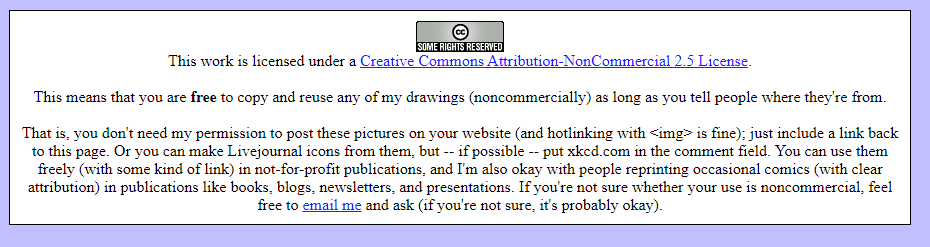
\includegraphics[width = \textwidth]{Copy-Right-Permissions/XKCD-permission.PNG}
    \caption{Copy right permission stated on the XKCD website}
    \label{fig:CR-XKCD}
\end{figure}

\subsection{Phdcomics}

On their website (http://phdcomics.com/about.php) they state

\textit{\textbf{Can I use one of your comics in my thesis/defense/website or graduate student newsletter?}
    We'll be happy to grant you permission, but you MUST e-mail us at questions(at)phdcomics.com to let us know how and which strips you are using (by sending this email, you obtain official permission to use the images). In all cases, the strips must have the following text printed next to them:}

\textit{	"Piled Higher and Deeper" by Jorge Cham www.phdcomics.com}

I have send them the email, and can  provide that proof if asked.

\subsection{Journal Article 1}

Here is were I present the permission from the Journal and co-authors for article 1 that I put into the thesis under Chapter \ref{sec-JA-Title1}.



\end{document}